\setchapterpreamble[ur][.6\textwidth]{%
\dictum[Fyodor Dostoyevsky, \textit{The Idiot} (1868--9)]{%
One can't understand everything at once, we can't begin with perfection all at once! In order to reach perfection one must begin by being ignorant of a great deal. And if we understand things too quickly, perhaps we shan't understand them thoroughly.}\vskip1em

\dictum[Voltaire a.k.a. Fran\c{c}ois-Marie Arouet, \textit{Candide} (1759)]{%
Si nous ne trouvons pas des choses agr\'eables, nous trouverons du moins des choses nouvelles.}\vskip1em}

\chapter[\texorpdfstring{Chapter 1 \\ General introduction}{Chapter 1 -- General introduction}]{General introduction}
\chaptermark{General introduction}
\label{chap:intro}
%%%%%%%%%%%%%%%%%%%%%%%%%%%%%%%%%%%%%%%%%%%%%%%%%%%%%%%%%%%%%%%%%%%%%%%%%%%%%%%%%%%%%%

%%%%%%%%%%%%%%%%%%%%%%%%%%%%%%%%%%%%%%%%%%%
\section{Variation in fitness}
\subsection{The origin of variation in evolutionary biology}
Understanding the causes of variation among living beings is at the heart of evolutionary questioning \parencite{Lynch1998, Wayne2006, Kruuk2014}. It is in fact its very starting point. Darwin opens his book \emph{the Origin of Species} with two chapters describing variability in domestic and wild organisms \parencite{Darwin1859}.
Building on these observations, Darwin then summarizes the evidence showing that variation within species is the fuel generating the astonishing diversity among species, but also the striking fit between organisms and their environment.

%causes of variation
These great answers immediately opened many more questions about the causes and consequences of variation, some of which remain not fully answered more than 150 years later. In particular, nineteenth century biologists struggled with the sources of variation within species, as is clear in \emph{the Origin of Species} itself:  ``\emph{Variability is governed by many unknown laws, of which correlated growth is probably the most important. Something, but how much we do not know, may be attributed to the definite action of the conditions of life. Some, perhaps a great, effect may be attributed to the increased use or disuse of parts}'' \parencite[p. 31][]{Darwin1859} \footnote{Alternatively, biologists dismissed this within-species variation by considering that species were arbitrary boundaries in a set or continuum of variation. Darwin did not attempt to define species, but by explaining how they originate, he made some definitions indefensible \parencite[][pp. 129-163]{Wilkins2009}.}. Of course, the effect of ageing was acknowledged and plastic responses to the environment were thought to be predominant \parencite{Wilkins2009}. Ageing and the environment does not always provide a satisfactory explanation for variation that appears within a population, however.
Furthermore, Darwinian arguments build on the observation of this special kind of inherited variation that can appear among siblings of a same litter, clutch or pod, and that is subsequently transmitted from parent to offspring \parencite[][Chapter 1]{Darwin1859}. The late nineteenth century was utterly ignorant of the sources of inherited variation within species. Only at the beginning of the twentieth century were the laws of inheritance progressively discovered and spread to the scientific community \parencite{Dietrich2006}. Four more decades saw these laws formalized into a unified scientific theory to understand variation within populations \parencite{Fisher1930}, and explained at the molecular level \parencite{Oswald1943, Watson1953}, thus closing the logical gap in Darwin's argument: Relatives resemble each other because they share similar gene versions on long strands of DNA, a molecule that is copied with high fidelity and transmitted from parent to offspring; There is variation among siblings because of the reshuffling and segregation of parental genes and, on occasions, because DNA mutates. 
The understanding of the causes of variation within species and populations has made terrific progresses and now fits elegantly in the broader evolutionary theory \parencite{Pigliucci2010}. Nevertheless, many aspects of the causes of variation are still to be refined or newly explored, especially in natural populations \parencite{Kruuk2014}. In particular, the relative importance of genes and the environment in the wild remains studied in only a few populations of a few species, taxonomically biased, and concerns a limited set of traits \parencite{Lynch1998, Postma2014}. 

Additional open research questions relate to the consequences of within-species variation. In particular, a lot of attention is paid to how genetic variation translates into adaptive evolution \parencite{Brookfield2016}.
Any trait that possesses genetic variation is evolvable, but it can evolve in an adaptive way only if the trait is subject to selection, be it artificial or natural. Selection occurs when the variation in the trait causes variation in \emph{fitness}. Before we discuss the specificity of the causes and consequences of variation in fitness, we must introduce this difficult concept.

\subsection{Variation in the definition of fitness}
There has been a great deal written about the concept of fitness, including multiple conflicting definitions, which ``\emph{is hardly surprising as every important scientific concept is difficult to understand from first principles, as for instance the notions of space and time, or energy and force}'' \parencite[p. 1358][]{Wagner2010}. I will not solve the question of the definition of fitness here, but I will try to make clear how the word is used in this thesis. To start with, in the past, there has been some confusion on whether fitness is a realized reproductive outcome or a propensity to reproduce \parencite{Brandon1984}. It is now rather consensual that the concept of fitness is more useful when it is defined as a propensity, that is, as an expected value that cannot be measured directly because of stochasticity \parencite{Brandon1984,Price1996,Krimbas2004} and we will follow this consensus. Fitness has been defined at the level of the genetic lineage \parencite[e.g.][]{Akc2016}, of the individual \parencite[e.g.][]{Cam2000}, of the genotype \parencite[e.g.][]{Steiner2012}, or of the population \parencite[e.g.][]{vanTienderen2000}. A propensity definition partly dissolves the problem of the level of the definition, since the expected reproductive outcome of a genotype is the same as the expected reproductive outcome of the individuals bearing this genotype, and the expected reproductive outcome of a population is the sum of the expectation of the reproductive outcome of its individuals. Here, we will consider fitness at the level of individuals, because they are the unit most easily observable and the primary target of natural selection.
More confusion on fitness comes from it being alternatively defined as the asymptotic number of descendants or as the contribution to the next generation \parencite{Wade2006}. Since we consider fitness at the level of individuals and because most of the work carried out is based on data covering about ten generations only, it is intuitive to consider fitness as the contribution to the next generation. Besides practical considerations, this choice allows for a clear, and conceptually crucial, distinction between selection, inheritance and evolution, that is blurred in asymptotic definitions \parencite{Fisher1930, Arnold1984}. 
A slightly contentious point is whether fitness should be defined as an absolute number of offspring \parencite{Wade2006} or a relative one \parencite{Rousset2004}, that is, whether ``relative fitness'' is a meaningful phrase or a tautological one. I feel like the relative definition is really closer to the interest of evolutionary biologists and avoids appending \emph{relative} to every occurrence of \emph{fitness}. Nevertheless the field massively favours the absolute definition and for the sake of consistency I attempted to yield to the convention (possibly with some inconsistencies). 
Finally, instead of a measure of reproductive success, relative fitness has recently been defined as the amount of information about the environment that populations accumulate by selection \parencite{Frank2012V}. I see great conceptual promises in this view, that brings together an essentialist use of the word \emph{fitness} and the scientific field of information theory. An information interpretation of fitness did not directly influence the work and is not necessary to understand it, but it might enlighten some of the results presented here, and evolutionary biology in general.
To sum up, we define the fitness of an individual as its expected number of descendant in the next generation.

\subsection{Causes and consequences of fitness variation in the wild}
Why is there variation in individual fitness? This question attracted a lot of research attention, because (i) genetic variation in fitness controls the pace of evolution within a population, and because (ii) an intuitive consequence of evolution is the erosion of genetic variation in fitness, thus making the presence of genetic variation in fitness paradoxical \parencite{Jones1987}. 
In this thesis, we will not deal with the second point, the fundamental question of appearance and maintenance of genetic variation in fitness, but rather with its proximal sources.
We will consider these proximal sources from two complementary angles. 

First in a descriptive approach, one can decompose variation in fitness into components of variation, without mention of the underlying mechanisms.
Apart from genetic variation, variation in fitness can also originate from variation in early-life, micro-environment \parencite{Turner2009}, or maternal effects \parencite{Wolf2009}. In addition, when working with wild sexual organisms, individual fitness as we defined it cannot be observed directly. Indeed, individuals are unique and their realized reproductive success does not equal their expected reproductive success. Therefore, researchers have to rely on fitness proxies, often realized reproductive success and survival, that contain a large stochastic component. Additive genetic variation in fitness is also the rate of evolution in fitness and sets the maximal rate of evolution \parencite{Fisher1930}. A variance decomposition approach is therefore useful to ascertain whether variation in fitness proxies is all stochastic and environmental or whether it hides genetic variation in fitness. In doing so, it determines how much adaptive evolution can be expected to happen within a population.

Second, in a more mechanistic approach, one can investigate what characteristics make some individuals fitter than others, that is what traits are under natural selection\footnote{In this thesis, unless mentioned otherwise, we consider \emph{sexual selection} as part of \emph{natural selection} and of \emph{selection}. Measuring sexual and natural selection separately, would certainly provide a finer understanding of the mechanisms of selection in the study population, but this was beyond the scope of this thesis. Nevertheless, the question was partly explored by \cite{Garcia-Navas2016} and \cite{Garcia-Navas2015a}.}. The study of natural selection in the wild took-off with the development of regression-based methods to accurately measure its strength and predict its effects \parencite{Lande1979, Lande1983}. Under some assumptions, the genetic change in response to selection on a trait is the product of a selection gradient and of additive genetic variation in that trait \parencite{Lush1937}. Therefore, by understanding what traits cause variation in fitness, one can predict what traits should evolve, as well as their direction and speed of evolution. 

The study of natural selection and adaptive evolution in the wild is very topical in the context of unprecedented rates of environmental changes induced by human activities \parencite{parmesan2006}. Anthropogenic changes provide the opportunity of natural experiments to evolutionary biologists \parencite{Altermatt2016, Brookfield2016}, but also come with societal concerns and an ever increasing urge to better understand and predict how living things respond to the selective pressures imposed by environmental changes \parencite{McCarty2001, Shaw2013}. This regain of focus has highlighted the gaps in the understanding of adaptation in natural populations: it is still challenging to predict, or even understand retrospectively, how natural populations respond to selective pressures \parencite{Merila2001, Tafani2013, Shaw2013, Brookfield2016}.

In order to study the evolutionary potential of wild populations and their response to selective pressure, it is necessary to measure genetic parameters. More specifically, one must determine whether the traits under selection are heritable, whether there is heritable variation in fitness and how what is the rate of genetic change for the traits of interest. 

%%%%%%%%%%%%%%%%%%%%%%%%%%%%%%%%%%%%%%%%%%%
\section{Measuring genetic variation}
\subsection{Looking up or down? Two philosophies}
How to measure and make sense of genetic variation?
For over a century, there have been two main approaches \parencite{Liedvogel2012}, that can grossly be traced back to the scientific controversy that opposed the Mendelians to the biometricians \parencite{Dietrich2006}, and summarized as ``bottom-up'' and ``top-down''. 
Bottom-up approaches, embodied by candidate gene and genome wide association studies, start from molecular data to infer the phenotypic effects of individual genetic loci. 
Top-down approaches, encompassed within quantitative genetics, attempt to decompose phenotypic variation into genetic variation and other sources of variation, based solely on phenotypic data and on some knowledge of the relatedness between individuals \parencite{Lynch1998}. 
Some pros and cons of both approaches are nicely illustrated by the confrontation of the quantitative genetics of mass with the genotyping of a candidate gene for mass. The former will be further developed in chapters \ref{chap:stasis} and \ref{chap:flusel} and we present it in a minimalist nutshell here: using a quantitative genetics \emph{animal model} \parencite{Henderson1950, Kruuk2004}, we estimated additive genetic variation in body mass and lifetime reproductive success. The latter is a side project of this PhD that does not appear in the other chapters, and we take the opportunity to present it below.

\subsection{A candidate gene for body mass: insights and limits}
We used a candidate gene approach \parencite{Fitzpatrick2005} to uncover the molecular mechanisms underlying variation in body mass. To date, the only candidate gene we fully analysed is an intronic region of the gene \emph{lepr}, which codes for the receptor to leptin. Leptin is a hormone known to regulate fat metabolism, energy expenditure and food intake, including in rodents \parencite{Houseknecht1998}.

We found a recessive allele (let call the recessive allele \emph{a}, and the dominant allele \emph{A}) associated with lighter individuals (Fig. \ref{fig:leprpheno}\textbf{A}). Homozygotes \emph{aa} were -2.9 g lighter (95\% credibility interval $[0.6;5.1]$), that is, 8\% lighter than the mean. On average, during their lifetime, these \emph{aa} individuals produced one third less offspring than the \emph{AA} individuals (Fig. \ref{fig:leprpheno}\textbf{B}). This strong difference in fitness is however not statistically significant, meaning that it could very well be the result of chance alone. These results suggest that some of the genetic variation in body mass is due to food intake and/or fat metabolism, which could not be sensed from the estimation of genetic variances and covariances. 
Based on such a strong phenotypic effect, \emph{lepr} could be called a major locus, but how much of the genetic variation does it explain?

\begin{figure}[ht]
	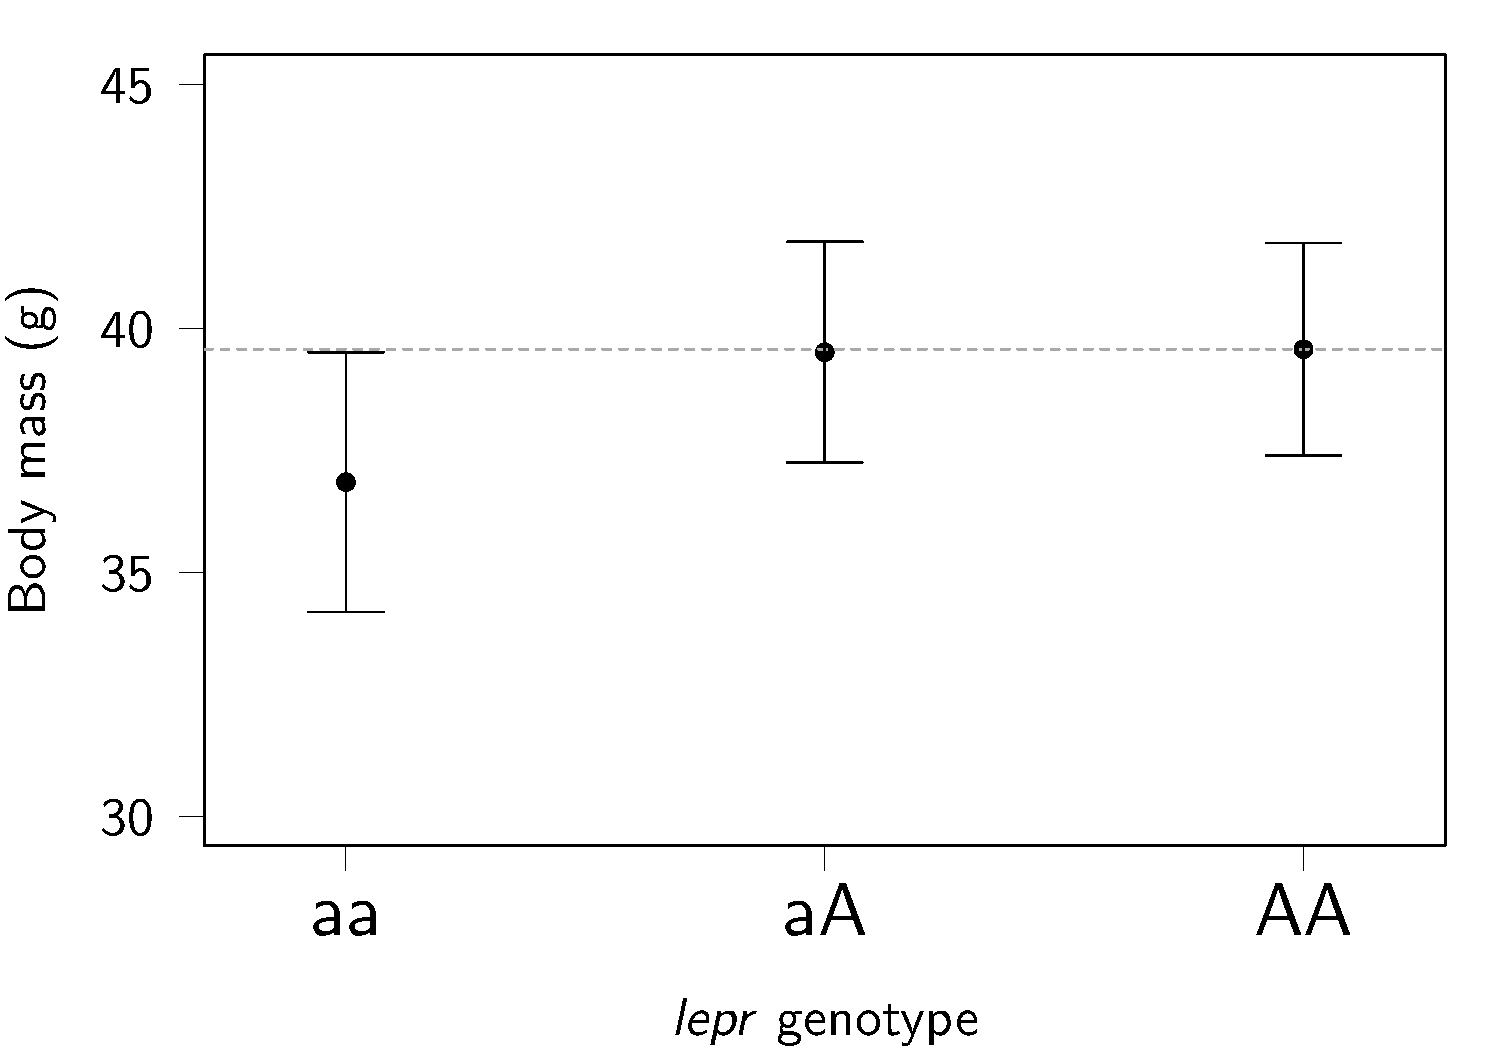
\includegraphics[width=0.5\textwidth]{FiguresGeneral/PhenoEffect-1}
	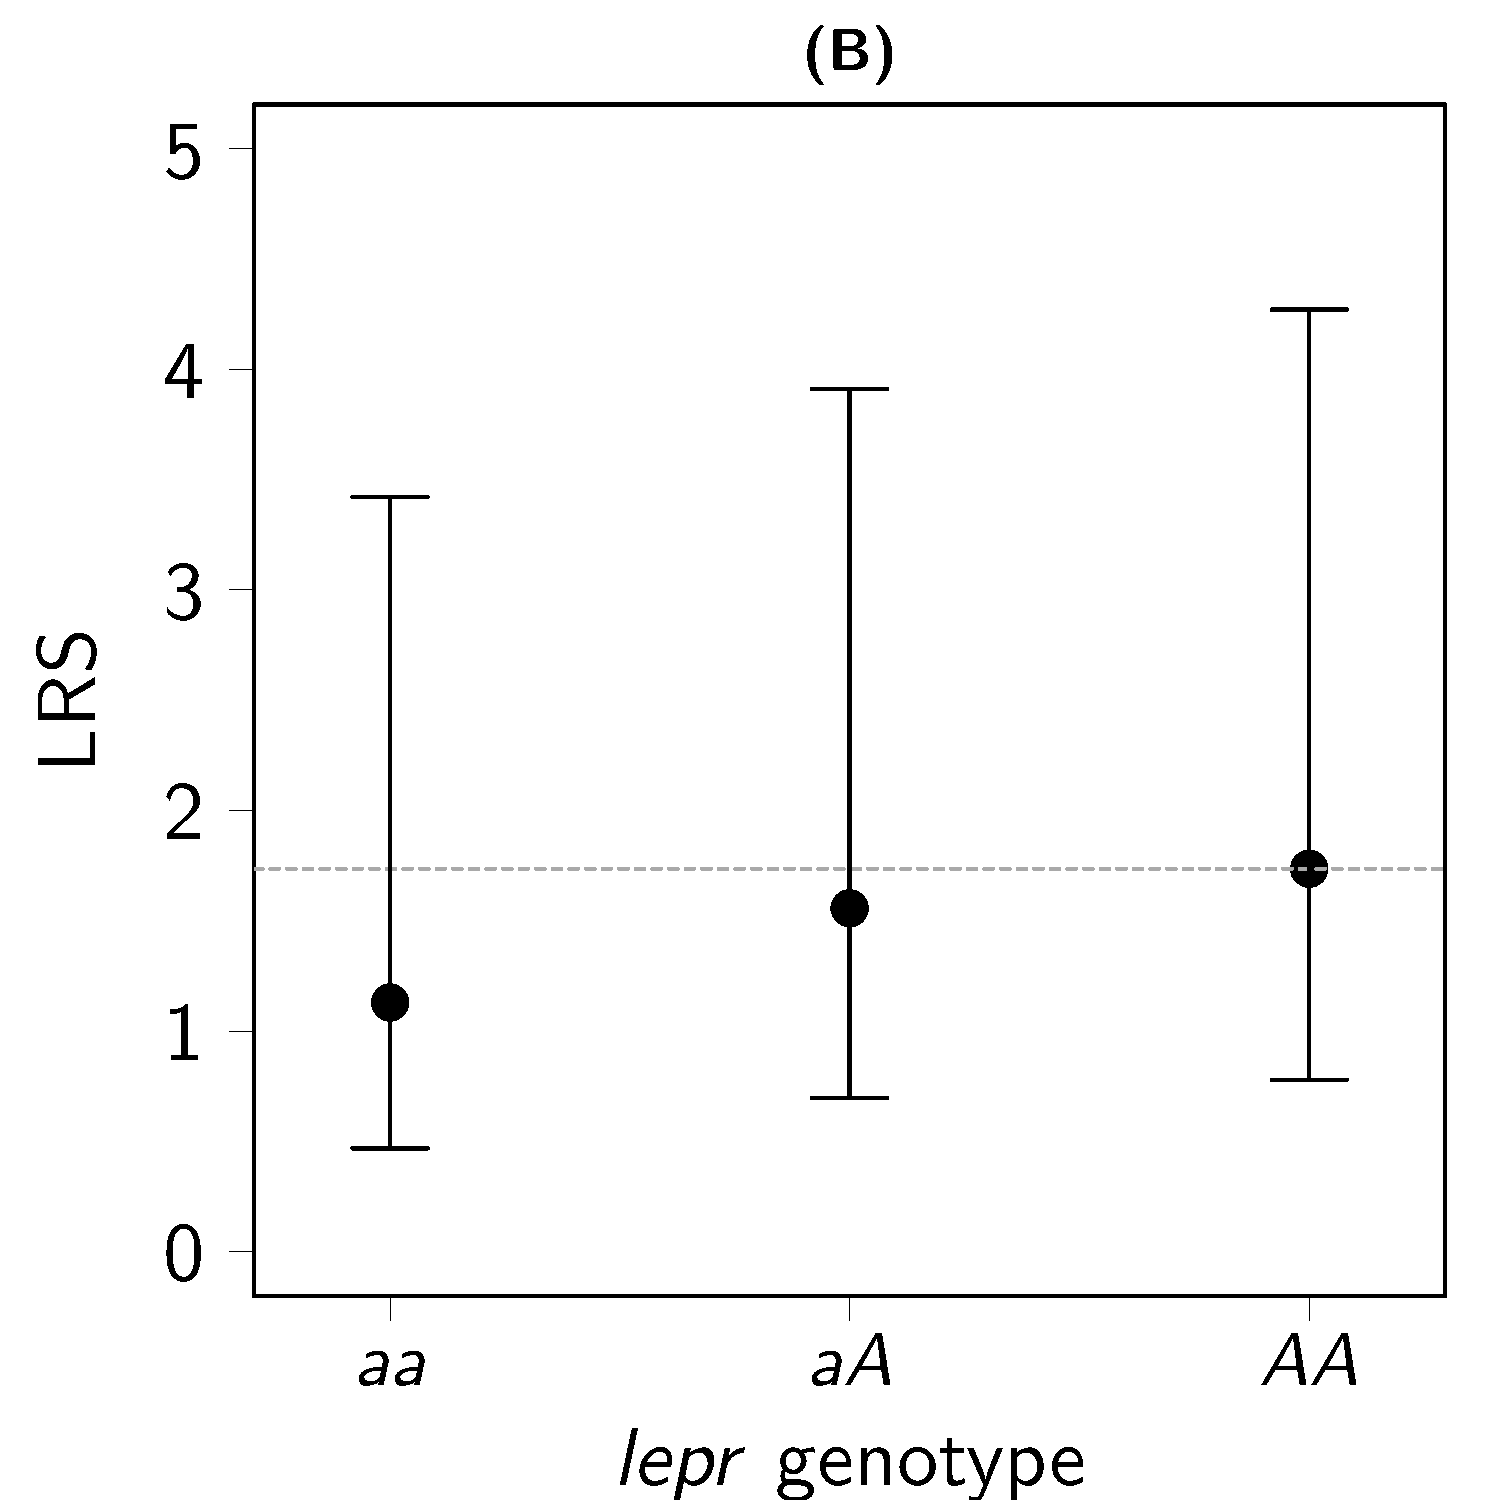
\includegraphics[width=0.5\textwidth]{FiguresGeneral/FitnessEffect-1}
	\caption{Body mass and lifetime reproductive success (LRS) as a function of \emph{lepr} genotypes. 
	(\textbf{A}) Expected body mass of snow voles bearing the three \emph{lepr} genotypes. The expectations and 95\% confidence intervals were predicted from a linear mixed model fitted to the 2311 mass measurement of 532 snow voles. The model accounted for sex, age, date of capture and their two-ways interactions, as well as year of capture and multiple measurements of the same individual.
	(\textbf{B}) Expected LRS of snow voles bearing the three \emph{lepr} genotypes. The expectations and 95\% confidence intervals were predicted from a Poisson generalized linear mixed model fitted to the LRS of 611 snow voles. The model accounted for inbreeding coefficient, year of birth and over-dispersion (using an observation-level random effect). For both panels, the dashed horizontal line projects the expected value of genotype \emph{AA} to ease comparison with \emph{Aa} and \emph{aa}.}
	\label{fig:leprpheno}
\end{figure}

Knowing the effect of the three genotypes and the allele frequencies one can compute analytically the additive genetic variances associated with a bi-allelic locus \parencite[][p77]{Fisher1941average,Lynch1998}. Thus, the additive genetic variances associated with \emph{lepr} are $0.052 \text{g}^2$ for body mass and $0.006 \text{pup}^2$ for lifetime reproductive success. For both traits, \emph{lepr} explains about 1\% of the additive genetic variation as estimated from an animal model. This is rather large for a single locus given that quantitative traits loci typically explain a fraction of a percent to a few percent of additive genetic variance (V$_\text{A}$), when they have a large enough sample size to mitigate Beavis effect \parencite{Flint2009,Jensen2014}.  Still, 1\% of V$_\text{A}$ is not sufficient to infer the evolutionary potential of the trait. Finally, genotyping many more markers, for instance using high-throughput sequencing \parencite{Goodwin2016}, is unlikely to improve this situation in the snow vole population. Generally, very large sample sizes and high-quality genomic resources are necessary to explain a biologically proportion of genetic variances \parencite{Bloom2013, Jensen2014}. For instance
183,727 individuals were necessary to find 180 QTL that jointly explained only 13\% of additive genetic variation in human body height \parencite{LangoAllen2010}.
High-throughput sequencing can also been used in a top-down way, that does not identify causal genetic variants, but instead quantifies the phenotypic variation jointly explained by all the genotyped markers. Thus, 3,925 individuals and 294,831 markers were able to explain 45\% of the genetic variation in human height \parencite{Yang2010}. This is much better, but given knowledge on the relatedness between individuals, quantitative genetics can estimate all the genetic variation in a phenotype, without any genotyping effort.

%Could we not use high-throughput sequencing techniques to explain a larger proportion of genetic variation, and at the same time identify the genes associated with phenoytpic variation and selection? 
%In theory we could, but in practice this avenue is still a rather laborious and expensive one \parencite{Goodwin2016}. The outcome is also uncertain: 
%The first objective, estimating genetic variances often requires huge sample sizes and number of markers and in general only a small fraction of V$_\text{A}$ is recovered \parencite{Bloom2013}. For instance, even in the most abundant and best known model organism, humans (\textit{Homo sapiens}, Linnaeus 1758), 
%sample sizes of over XXX were necessary to explain 
%XX\% of variation in body mass. 
%Such progresses were accomplished by increasing sample sizes by several order of magnitude and developing Neither can be achieved in small populations of non-model organisms.

%The second objective, identifying the genetic mechanisms of variation and selection, in small populations the number of genetic loci that can be identified with statistical significance can be limited by the problem of multiple comparisons, although solutions are emerging. Moreover, the genotype/phenotype map can hardly be understood from a fully bottom-up approach because of pervasive interactions among genes and with their environment \parencite{Pigliucci2009}. 

To conclude, bottom-up approaches can better unravel the molecular mechanisms underlying phenotypes. By opening the black box of what mechanisms make up a phenotype, they can identify what is most crucial in a phenotype, how it is linked to the environment and what is the target of natural selection \parencite{DeJong2014}. Moreover, they contribute to building a genotype-phenotype map, a long lasting challenge in evolutionary biology \parencite{Kirschner2010}.
On the other hand, quantitative genetics lump all the effects of individual genes and their interactions into only a few parameters, non-informative about the underlying genetic architecture \parencite{Mackay2001,Nietlisbach2015,Huang041434}.  This summarized estimation provides simple and direct measures of genetic parameters. Quantitative genetics work directly on the phenotype which is the target of selection, and the source of ecological interactions. They therefore provide simple measures of genetic parameters that can directly be interpreted within the ecology of organisms.
This thesis is concerned with the genetics and evolution at the level of organisms, in relation to their environment, and accordingly, most of my work relies on quantitative genetics.

%\subsection{Consequences of variation in fitness}
%%consequences of variation
%Additional questions relate to the consequences of within-species variation.
%Furthermore, within-population variation is relevant to the demographic response to environmental changes, either through the direct effect of phenotypic variation (including genetic variation) \parencite{Kendall2011, vindenes2015, Plard2016}, or indirectly, following genetic changes \parencite{Chevin2010a, Turcotte2011, Schiffers2013a}. Once more, many questions remain open, which is not surprising given that this focus took off only in the last decade. Theory is being developed to describe the joined evolutionary and demographic dynamics in response to environmental change \parencite{Chevin2010a, Childs2016}, but there is still little confrontation to empirical data \parencite{Chevin2012, Gonzalez2013a}, and how evolution and demography interact in natural populations remains unclear \parencite{Charmantier2014climate, Gonzalez2013a}. 


%%%%%%%%%%%%%%%%%%%%%%%%%%%%%%%%%%%%%%%%%%%
\section{This thesis}
\subsection{Objectives}
In this thesis, I investigate the proximal causes of individual-level variation in fitness, and the consequences of this variation at the population level. This thesis aims at better measuring and better understanding selection and evolution in the wild. It examines the relative importance of stochasticity and selection in shaping reproductive success and survival, disentangles evolutionary from plastic changes and explores the link between selection and evolution. These questions are addressed using a combination of computer simulations and of data from the long-term individual-based monitoring of a snow vole population.

\subsection{Snow voles in Churwalden}
% Species
The snow vole (\textit{Chionomys nivalis}, Martins 1842) is a medium-sized rodent, its adult body size ranges from 10 to 14 cm, without the tail (5 to 7.5 cm long). Contrary to a widespread intuition, snow voles are not white (Fig. \ref{fig:juvvole}). Instead, the fur colour of the upper-parts varies from light to dark taupe grey, sometimes tinted with brown or dark red. The misconception about color highlights that the species could favourably be renamed \emph{rock vole}: it is a rock, rather than a snow, specialist \parencite{Luque-larena2002} and might be associated with high elevations only because rocky areas are more widespread there. It is sparsely distributed across southern Europe and Asia Minor, from sea level up to 4000 m of elevation \parencite{Janeau1997}.
\begin{figure}[ht]
	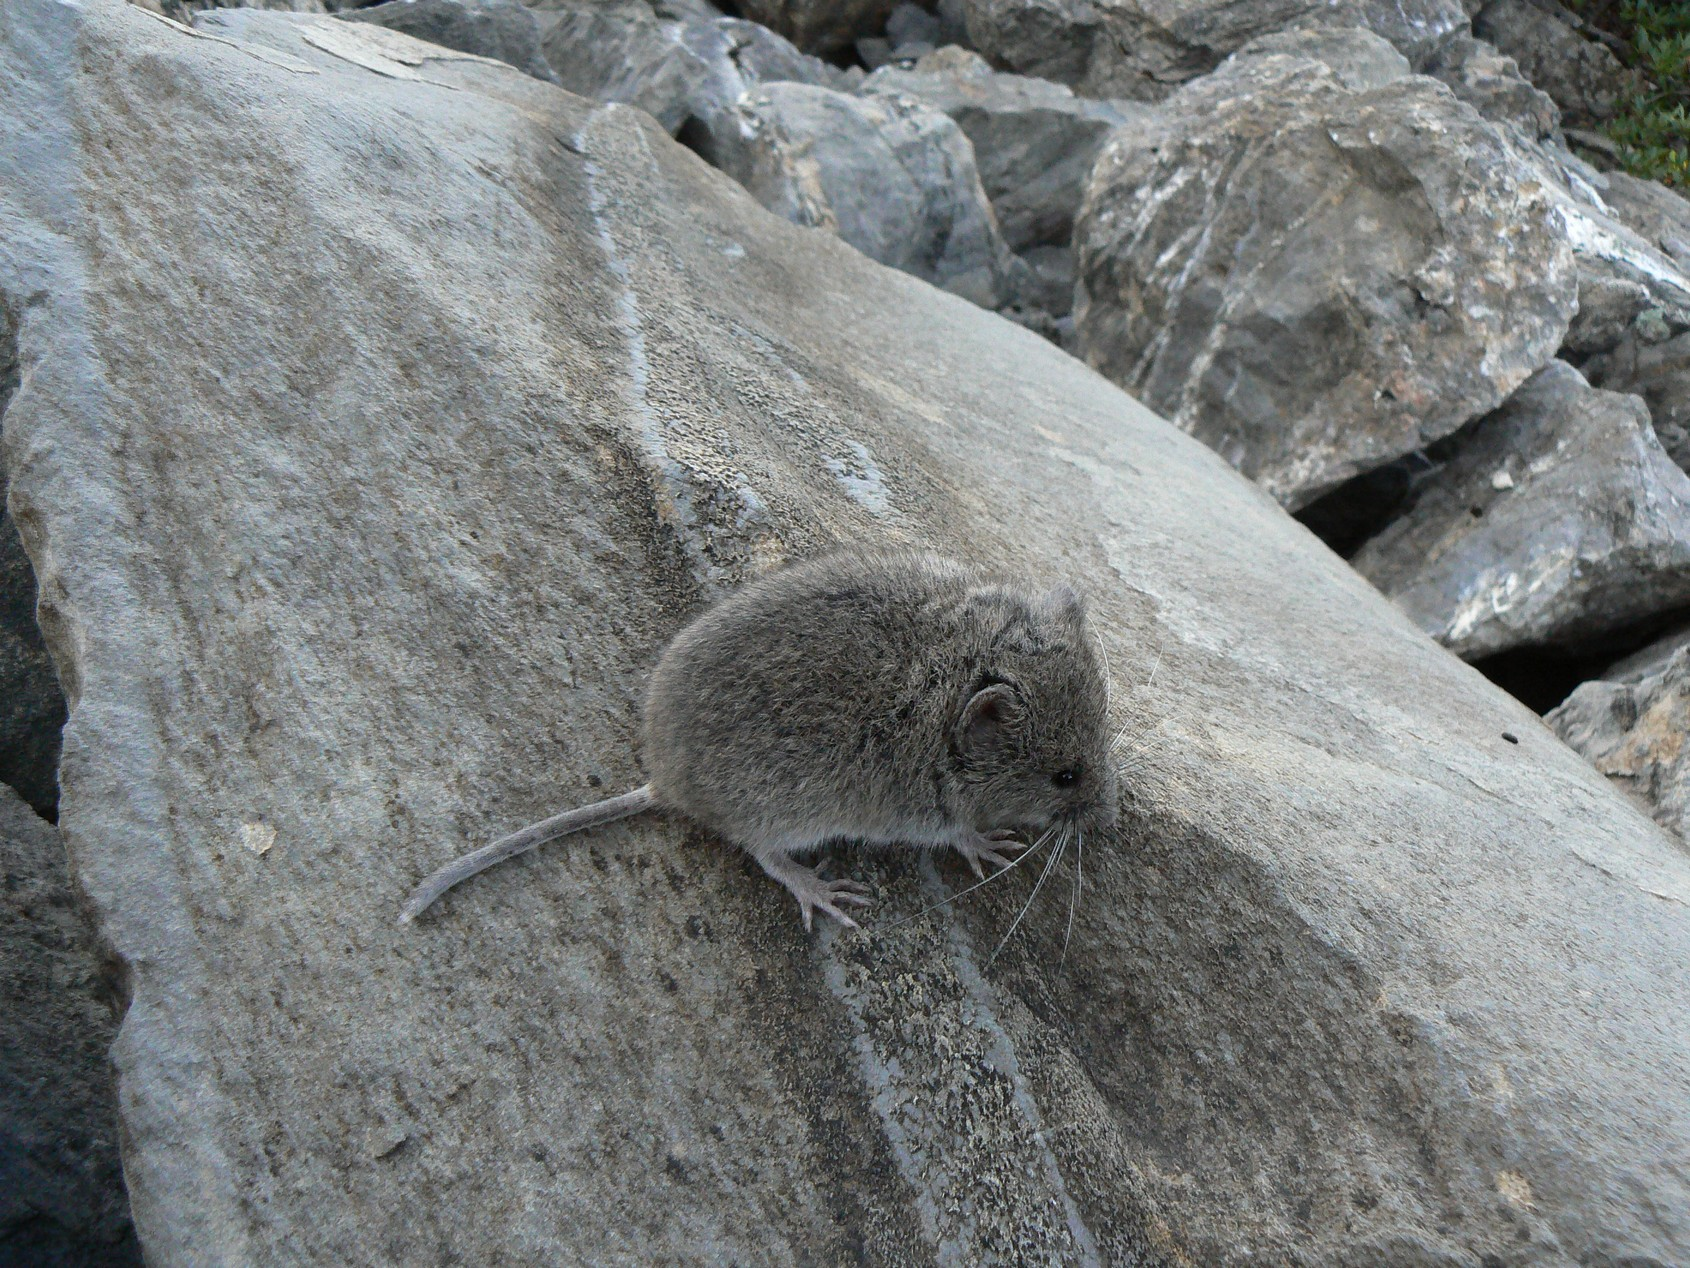
\includegraphics[width=0.49\textwidth]{FiguresGeneral/juvvole.JPG}
	\hspace{0.02\textwidth}
	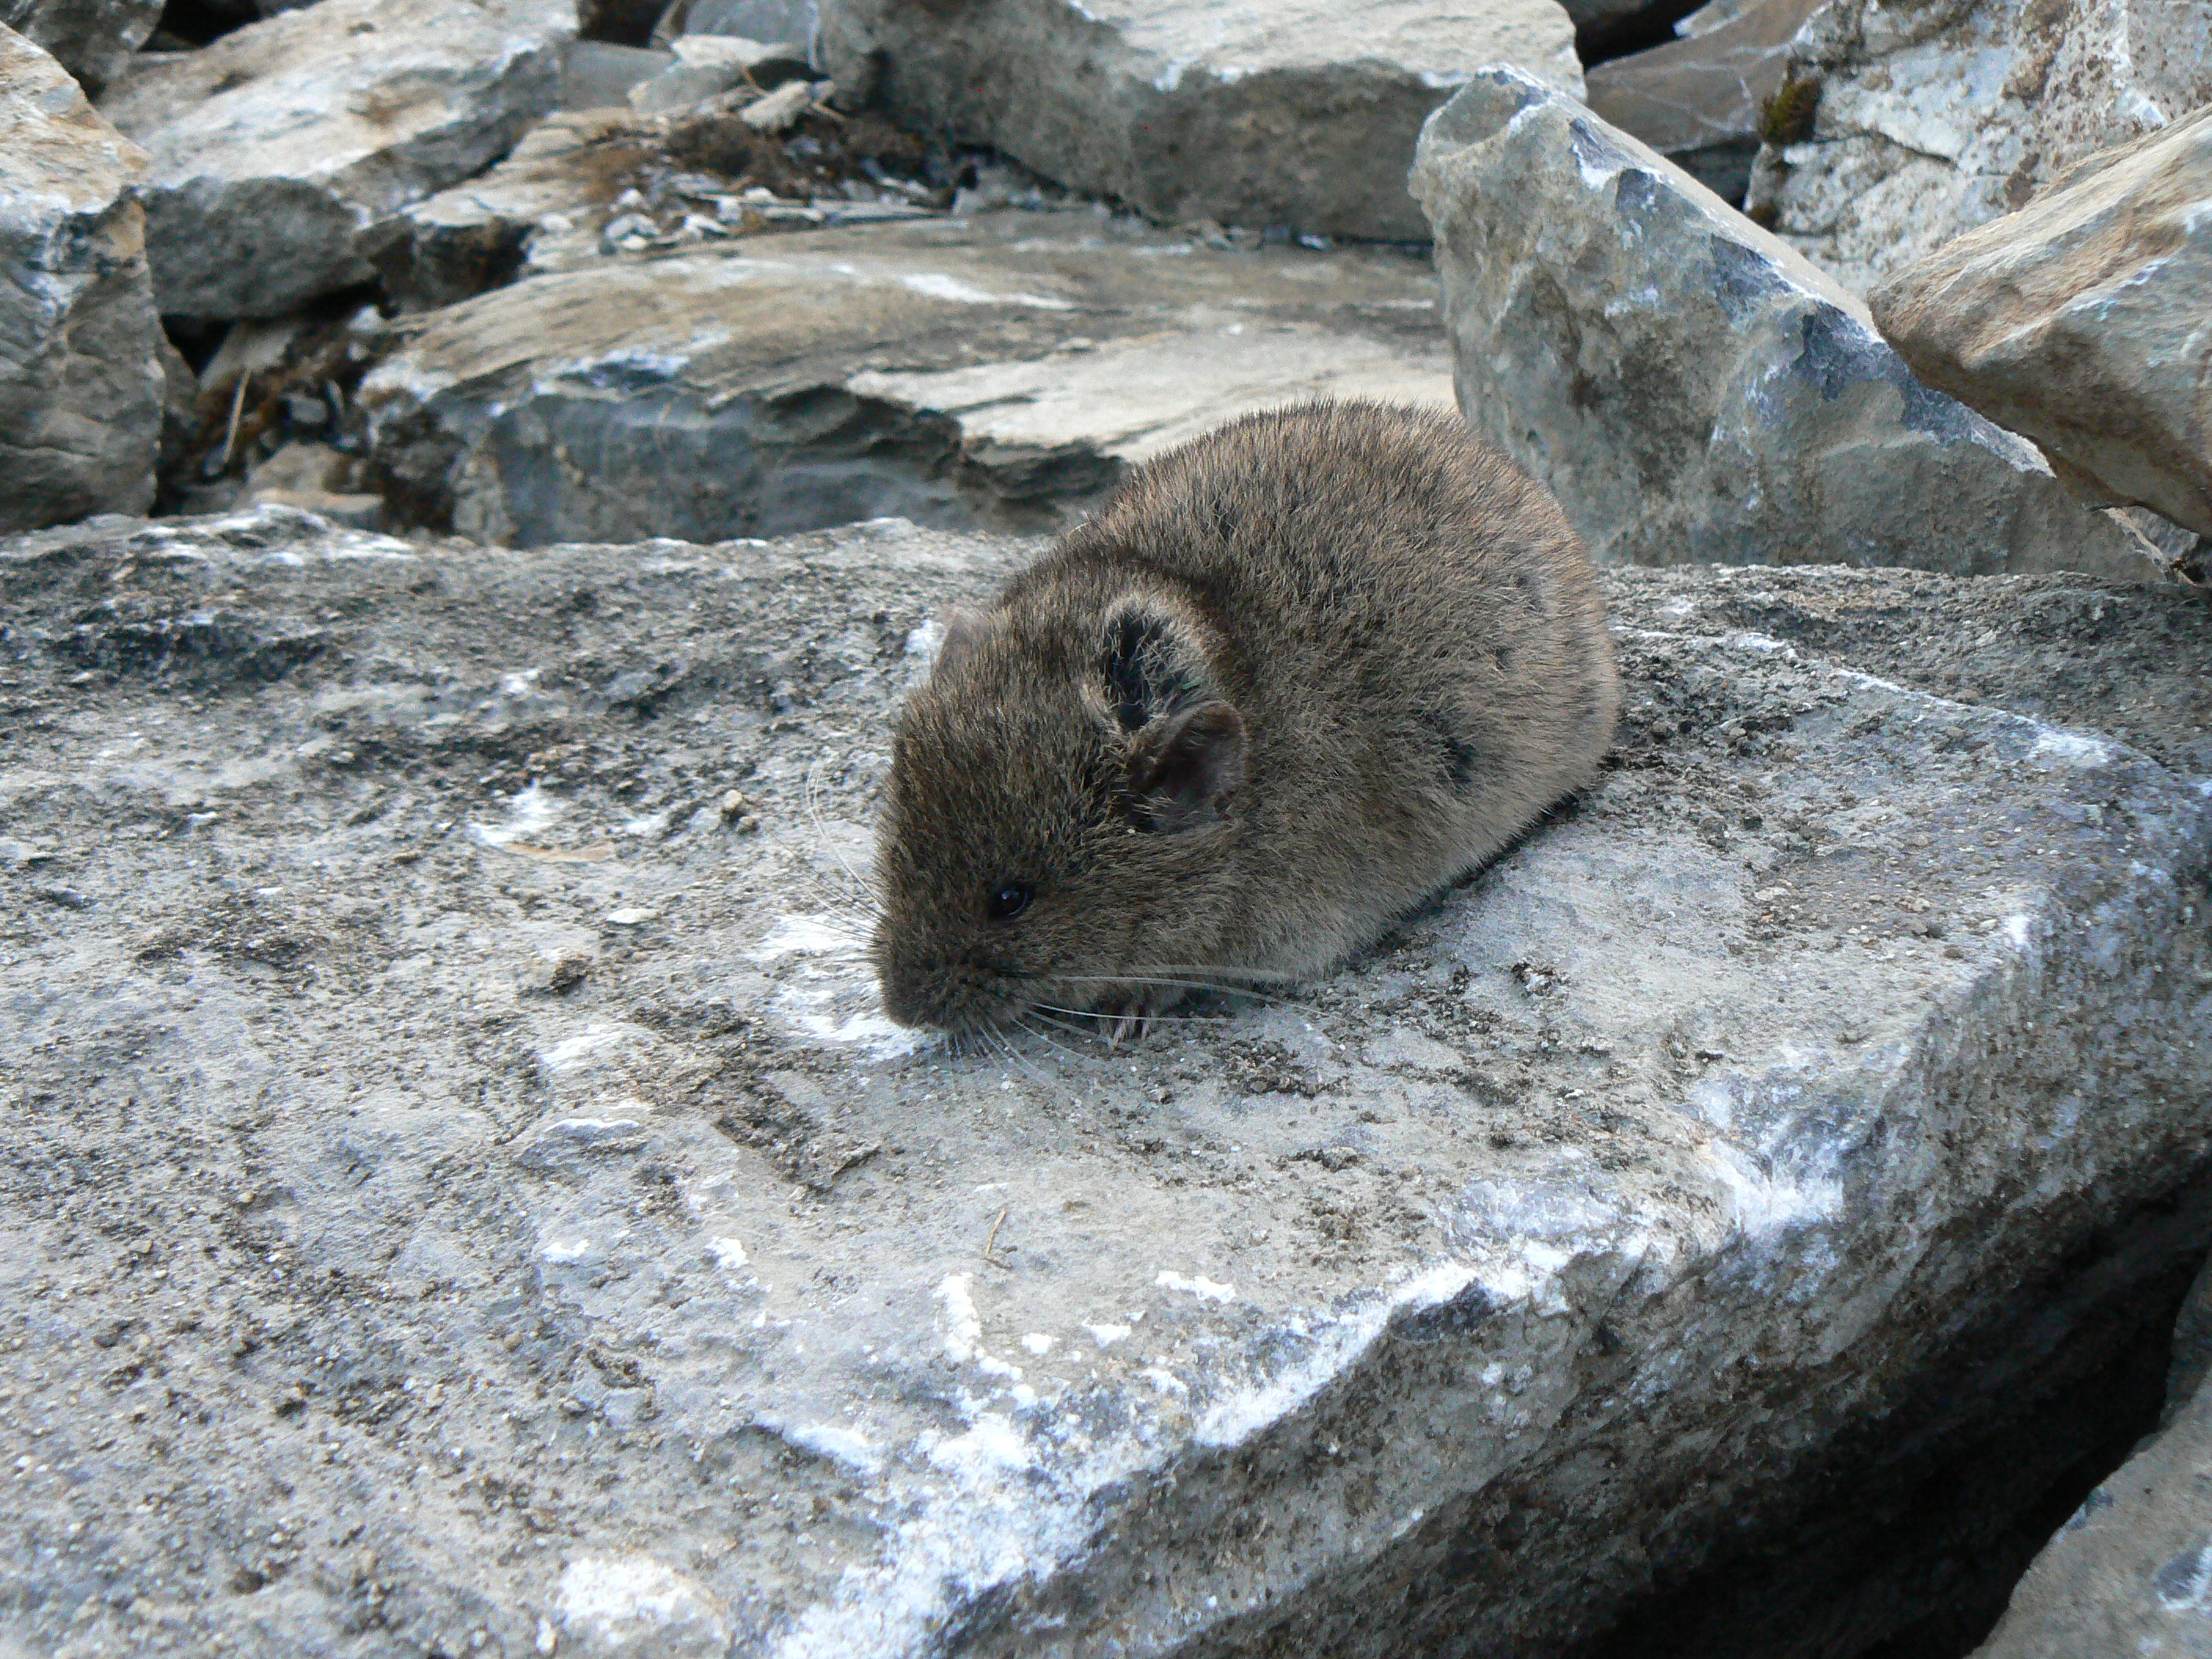
\includegraphics[width=0.49\textwidth]{FiguresGeneral/advole.JPG}
	\caption{Juvenile (left picture) and adult (right picture) snow voles in their habitat in Churwalden, Switzerland. Juveniles always lack the brown hue generally found in adults. Neither adults nor juveniles are white.}
	\label{fig:juvvole}
\end{figure}

Snow voles excavate burrows under the rocks, but can also use natural clefts between rocks, sometimes carrying small stones to build walls \parencite{Niederer2008}. A burrow consists of tunnels connecting chambers, one for the nest and multiple ones to stock dry plants \parencite{Janeau1997}. The species is not known to hibernate and is therefore exposed to harsh winter conditions in its high-elevation range. 
Adult females actively defend small territories against non-relatives, and tend to form matrilineal clusters of territories, whereas adult males wander, and fight, across large overlapping home-ranges \parencite{Luque-larena2004, Garcia-Navas2016}. The matting system is promiscuous and a same litter can be sired by multiple males. Females normally produce 1 to 4 litters of 1 to 5 pups between May and September. Juveniles generally do not reproduce in their first civil year. 
Although they can eat flour worms in the lab, there is no evidence that snow voles are not strictly herbivorous in the wild \parencite{Janeau1997}. In the Swiss Alps, snow voles suffer predation from red foxes, stoats, various owls and corvids, and parasitism from flees, lices and ticks \parencite{Janeau1997, Martinoli2001}.

% Population, characteristics
The study area is located by the Churer Joch, Churwalden, in the Swiss canton Graub\"unden (coordinates $46^{\circ}$48' N, $9^{\circ}$34' E), and covers about 5 ha between 1980 m and 2100 m above sea level. It consist of a west-exposed scree interspersed with small coniferous trees and with patches of alpine meadow. The study area is demarcated by extensive meadows to the south and to the north, by a coniferous forest to the west and by cliff to the east (Fig. ref{fig:landscape}). 
\begin{figure}[ht]
	\includegraphics[width=1\textwidth]{FiguresGeneral/DSC_2111viewontaliflue}
	\caption{Distant view of the field site, taken from the west. The trapped area covers about a fifth of the width and a tenth of the height of the picture and is located in the centre. This scree is surrounded by a forest, a cliff and meadows.}
	\label{fig:landscape}
\end{figure}

Another scree, called Wolfgruoben, offers about 1 ha of favourable habitat, starting 300 m north-east to the monitored area. Wolfgruoben was trapped in 2008 and 2013. The snow vole density was rather low, with on average five captures per night of trapping, versus 18 on the main study area. More habitat favourable to snow voles can be found 2 Km to the south. The study population is moderately isolated and receives 5 to 10 immigrants per year, on a total of 60 to 180 individuals \parencite{Garcia-Navas2016}. 

% Monitoring and history
The monitoring of this snow vole population was initiated in 2006 by Dr. Peter W. Wandeler. Dr. Erik Postma took the monitoring over in 2012, but the protocol has remained practically unchanged. This thesis contains data collected up to the year 2015.
\begin{figure}[ht]
	\begin{tikzpicture}
		\node (pic) at (0,0) {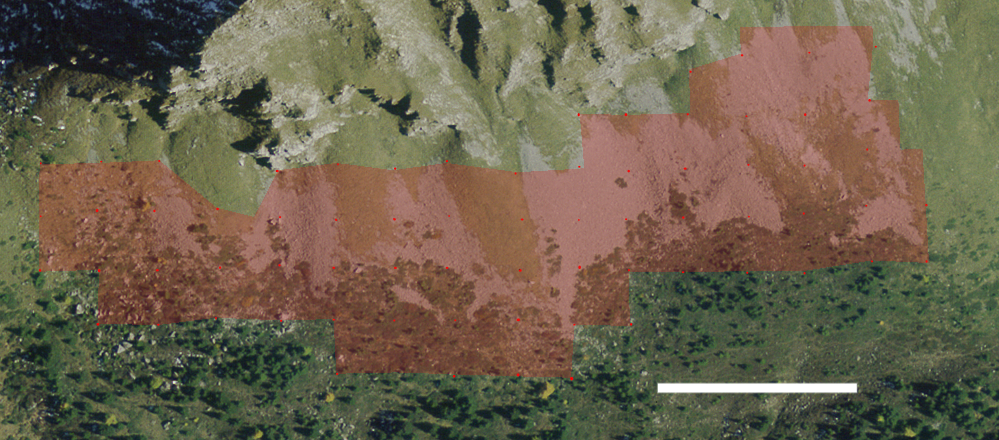
\includegraphics[width=1\textwidth]{FiguresGeneral/fieldposts2.PNG}};
		\draw[<-, ultra thick, color=white,>=stealth] (6.5,-2.5)--(7.5,-2.65);
		\node (n) at (6.3,-2.4) {\color{white}{N}};
		\draw[ultra thick, color=black] (2.52,-2.59)--(2.52,-2.75)--(5.68,-2.75)--(5.68,-2.59);
		\node (m) at (4.1,-3) {\color{white}{100 m}};
		%\draw[ultra thick, color=black] (2.52,-2.75)--(2.52,-2.65);
		%\draw[ultra thick, color=black] (5.68,-2.75)--(5.68,-2.65);
	\end{tikzpicture}
	\caption{Orthophoto of the study site, from 2008. The red shading indicates the approximate area where traps are set.}
	\label{fig:fieldarea}
\end{figure}
Every year from 2006 to 2016, snow voles were life-trapped multiple times between late May and early October. Traps were set during the day, opened around sunset and checked the next morning. 
For every snow vole capture \footnote{Other species (bank voles, pine voles, wood mice, stoats, black salamanders, slugs\dots) were released without taking measurements.}, we recorded sex, age, body mass, body length, tail length, date, location and signs of reproductive activity (pregnancy, lactation, swollen scrotum). 
In addition, all newly-captured snow voles were individually marked and genotyped for 18 microsatellites \parencite{Wandeler2008}. Based on the autosomal microsatellite genotypes, we reconstruct the pedigree of the population. This pedigree is the raw material for most of the work carried out during this thesis. In particular, the pedigree is used to define reproductive success, as well as to estimate the relatedness between all pairs of individuals. These two statistics are essential to estimate selection, fitness and genetic variation. 


\subsection{Thesis outline}

In natural populations, fitness is generally measured using individual measures of reproductive success and survival. These proxies are not fitness itself and their variation is largely stochastic, leading some authors to doubt that there is any significant variation in fitness in natural populations. Recent methodological developments appeared to support the view that variation in reproduction and survival was purely stochastic, and suggested that the potential for selection and evolution in the wild was largely over-estimated. In \textbf{Chapter \ref{chap:dynhet}} I examine these methods and, based on computer simulations, demonstrate that they lack statistical power to detect latent variation in fitness components. Using an alternative approach we show the presence of significant variation in the propensity of reproductive success in the snow vole population, thereby showing some potential for selection and adaptive evolution in this population. We also attempt to clarify some conceptual misunderstandings between the proponents of the two methodological schools. 

A similar attempt motivated \textbf{chapter \ref{chap:decpop}}, where, with collaborators from different methodological schools, we review and compare four frameworks to disentangle the causes of phenotypic changes. In particular, these frameworks differ in their estimation of the relative roles of plasticity, demography and genetic change. Based on computer simulations and on mathematical comparisons, we show that the discrepancies between the frameworks primarily originates from different definitions of the components of change. Nevertheless, one of these frameworks, the quantitative genetics \emph{animal model}, stands out as the only framework able to estimate genetic change and the response to selection (that is, the trans-generational consequence of variation in fitness). I relied heavily on this framework for the two next chapters.  

In \textbf{chapter \ref{chap:stasis}}, I explore the reasons of the mismatch between apparent phenotypic selection, phenotypic change and genetic change for body mass. I describe one of the first case of contemporary evolution of a quantitative trait in the wild and show that this genetic change is adaptive. Both the evolution and the selective pressure responsible for it are invisible to purely phenotypic approaches, however. Using multivariate animal models, we identify the main component of selection as juvenile viability. I then infer that the target of selection is potential adult mass in juveniles and that selection is related to a recent change in climatic conditions. 

The previous chapter considered selection and evolution averaged over the whole study period, without considering their temporal dynamic within the period. The fluctuation of selection is thought to be a major determinant of the rate of evolution, and a process to consider to understand adaptation in the wild. 
Nevertheless, unbiased measures of the variation of selection are rare and of the coupling between variation in selection and variation in evolution has been largely ignored. \textbf{Chapter \ref{chap:flusel}} shows that selection fluctuates in the study population, mainly due to variation in fertility selection. The rate of adaptive evolution is, however, remarkably constant, because viability selection, the driver of body mass evolution, does not vary. In this case the fluctuation of selection is evolutionary irrelevant. These two last chapters highlight the dangers of relying on phenotypic estimates of selection to understand the evolutionary dynamics of natural populations.

Finally, in \textbf{chapter \ref{chap:discu}}, I summarize the progresses made during this PhD on the understanding of natural populations and discuss some of the remaining challenges and future working directions.

\printbibliography[heading=subbibliography]

